\documentclass{article}

\usepackage[english]{babel}
\usepackage{graphicx}
\usepackage{blindtext}
\usepackage{array}

\usepackage[letterpaper,top=2cm,bottom=2cm,left=3cm,right=3cm,marginparwidth=1.75cm]{geometry}

\usepackage[colorlinks=true, allcolors=blue]{hyperref}

\begin{document}

\title {\textbf{Melanoma Detection with Deep Learning} \\[1ex] \large Science Depth Study}
\author{k4yp}
\date{}
\maketitle
\vspace{1in}
\begin{center}
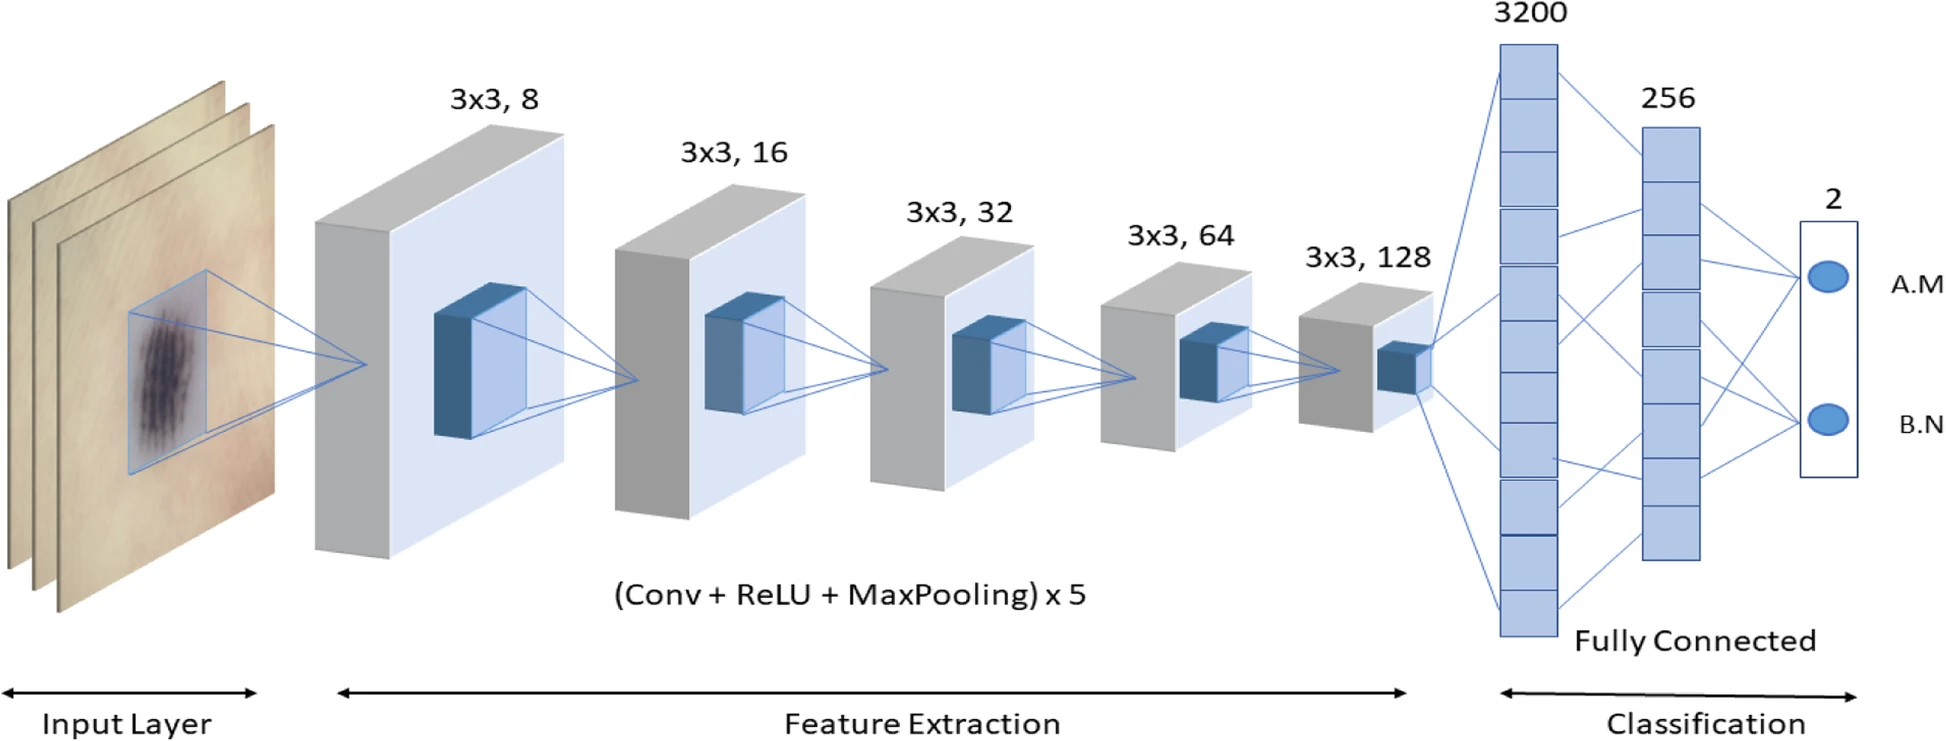
\includegraphics[width=14cm]{intro.png}
\end{center}
\newpage

\renewcommand{\baselinestretch}{2}\normalsize
\tableofcontents
\renewcommand{\baselinestretch}{1.1}\normalsize

\newpage

\subsection{Introduction}
Melanoma accounts for only 1\% of skin cancers but causes a majority of skin cancer deaths (American Cancer Society, 2019).  The Australian Institute of Health and Welfare estimates over 16,878 new melanoma cases will be diagnosed in 2021. It is also estimated that 1,315 people diagnosed with melanoma will die from the disease. Similar to other cancers, early and correct detection can drastically improve the effectiveness of treatment. Currently, dermatologists evaluate all skin lesions on a patient to identify outliers that are most likely to be melanoma. Dermatologists could enhance their diagnostic accuracy with the help of Deep Learning algorithms trained to identify Melanoma. If successful, Dermatologists would be able to make more accurate predictions and treat patients more effectively. Although Melanoma is a deadly disease, if detected early, the majority of skin lesions can be removed with minor surgery. Deep Learning algorithms that automate the diagnosis of melanoma could greatly increase a dermatologist's accuracy. Improved melanoma detection has the potential to benefit millions of people and save thousands of lives.

\begin{center}
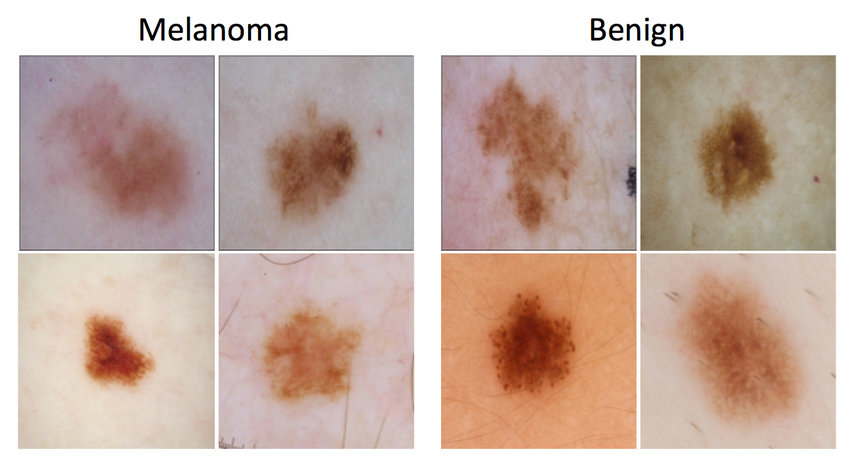
\includegraphics[width=12cm]{examples.png}
\end{center}
Figure 0: Examples of malignant and benign skin regions (ResearchGate, Example lesion classification of dermoscopic images - Noel Codella)

\subsection{Aim}
Dermatologists on average have a 67.4\% to 76.1\% chance of correctly predicting melanoma based on clinical and dermoscopic images (Dermatology Practical & Conceptual, 2021). The aim of this experiment is to determine whether Deep Learning can predict melanoma with a higher accuracy than dermatologists.

\subsection{Hypothesis}
The ResNet50 Deep Learning model will be able to predict melanoma in skin lesion images with a higher accuracy than dermatologists, due to the large training dataset and the complexity of the model.

\subsection{Variables}
\begin{itemize}
\item[\textbf{-}] Independent Variable - Number of epochs used for training the model 
\item[\textbf{-}] Dependent Variable - Accuracy of melanoma prediction (on validation data)
\item[\textbf{-}] Control Variable - Accuracy of melanoma detection from human dermatologists 
\end{itemize}

\subsection{Materials}
A laptop with a stable internet connection, where you can run the code in a free online cloud  virtual machine like Google Collaboratory or an interactive Kaggle Notebook. For offline use a computer with Python 3.9 or higher installed and a NVIDIA graphics card for better performance and integration with CUDA. The dataset used is the \href{https://www.nature.com/articles/sdata2018161}{HAM10k Dermatoscopic Image Collection from Harvard}. An augmented version is being used that balances the melanoma to non-melanoma samples using data augmentation.

\begin{itemize}
\item[\textbf{-}] Link to interactive notebook on Kaggle: \href{https://www.kaggle.com/code/keypos/resnet50-melanoma-classification}{https://www.kaggle.com/code/keypos/resnet50-melanoma-classification}

\item[\textbf{-}] Link to augmented Kaggle dataset: \href{https://www.kaggle.com/datasets/drscarlat/melanoma}{https://www.kaggle.com/datasets/drscarlat/melanoma}

\item[\textbf{-}] Link to direct source code on GitHub:
\href{https://github.com/keyp0s/melanoma/blob/main/resnet50-melanoma-classification.ipynb}{https://github.com/k4yp/melanoma/blob/main/resnet50-melanoma-classification.ipynb}
\end{itemize}

\subsection{Method}
ResNet50 is being used as the base model. The model consists of 48 convolution layers which makes it exceptional at image recognition and classification. The model is then trained on over 10,000 augmented images from the HAM10k dataset. These images will slowly train the model in a series of runs called epochs. In esence the model starts out with no prior knowledge and is fed one image at a time. At the beginning the predictions are almost random. When the model predicts an image wrong it takes that feedback and through backpropagation adjusts its parameters. At its core the model distinguishes features of melanoma lesions leading to the accuracy of the model exponentially increasing until it flattens off and peaks. If the model is trained for too many epochs it will start to over-fit on the data. This is when the model becomes extremely accurate at identifying the data it has been trained on but useless at predicting images it has not seen in training. This is a common issue in Deep Learning so multiple runs of different epochs will be tested to find the optimal training amount. A separate dataset of 3000 images the model has not been trained on will be used to test the models accuracy.

\begin{center}
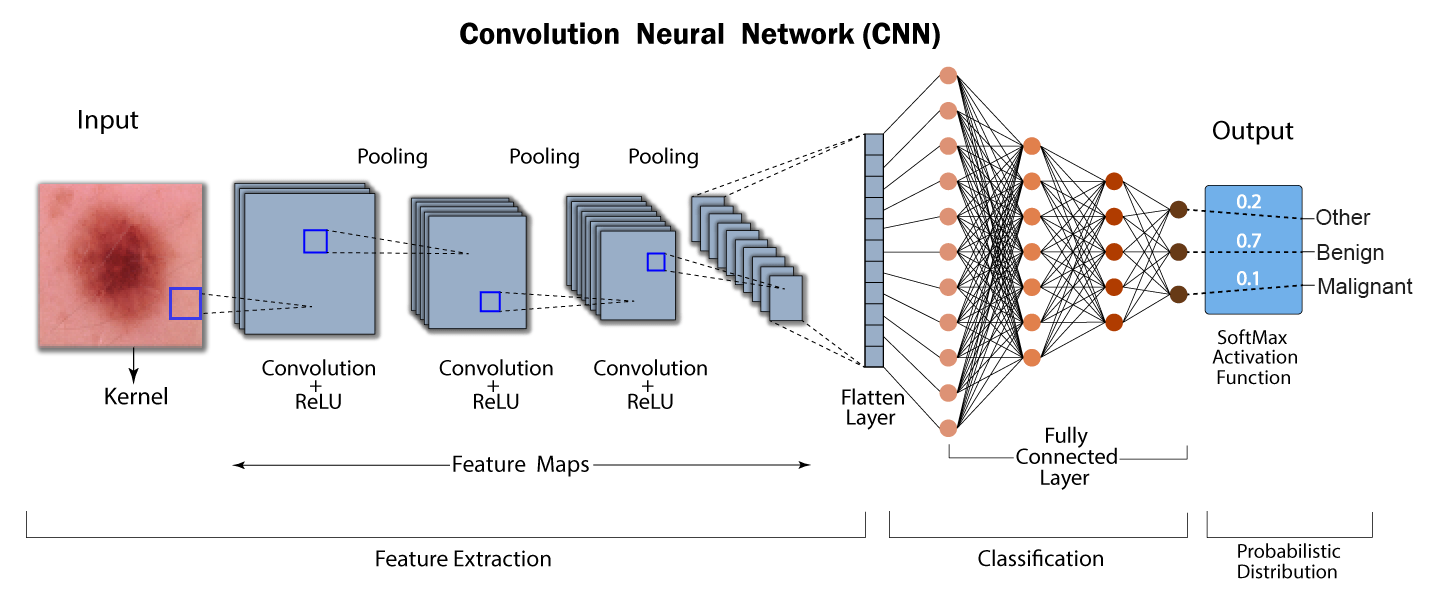
\includegraphics[width=15cm]{cnn.png}
\end{center}
Figure 1: Example of Convolutional Neural Network Architecture
\subsection*{Results}
After training for 1 epoch the model predicted melanoma on the test data with an accuracy of 88.9\%. From there the model improved as the epochs increased but still stayed relatively consistent. The model predicted most images in a binary fashion with most samples either being 100\% or 0\% melanoma (Figure 3). Though some images were predicted incorrectly (Figure 4). The model did surpass the initial 76.1\% baseline accuracy by Dermatologists.

\begin{center}
\begin{tabular}{ | m{2cm} | m{4cm}| } 
\hline
Epochs &
Accuracy on test data \\
\hline
1 &
88.9\% \\
\hline
2 &
91.3\% \\
\hline
4 &
91.8\% \\
\hline
8 &
92.4\% \\
\hline
16 &
92.5\% \\
\hline
32 &
93.2\% \\
\hline
64 &
93.4\% \\ 
\hline
\end{tabular}
\end{center}

\begin{center}
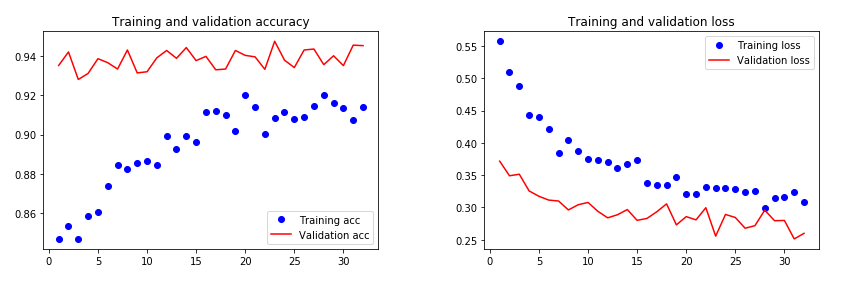
\includegraphics[width=15cm]{acc.png}
\end{center}
Figure 2: Training accuracy and loss with 32 epochs of training

\vspace{1cm}

\begin{minipage}{16cm}
  \centering
  \raisebox{-0.5\height}{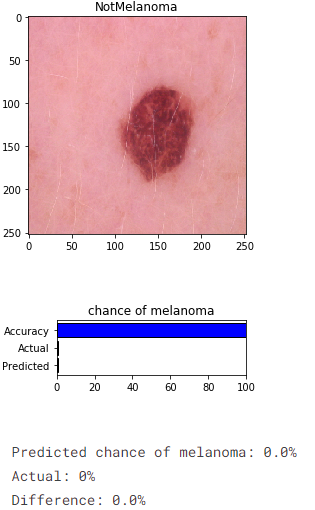
\includegraphics[width=5cm]{results01.png}}
  \hspace*{2cm}
  \raisebox{-0.5\height}{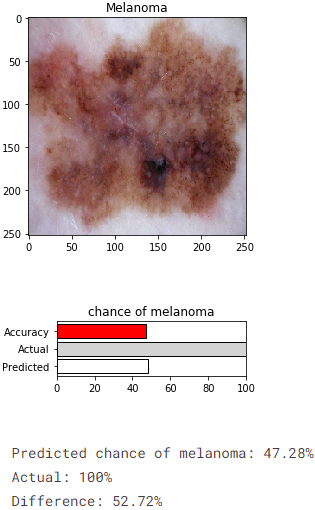
\includegraphics[width=5cm]{results02.png}}
\end{minipage}

\vspace{1cm}

Figure 3 (on left): Correct prediction of benign skin lesion

Figure 4 (on right): Incorrect prediction of melanoma skin lesion

\vspace{0.5cm}

\subsection{Discussion}
The hypothesis was proven true with the Deep Learning model predicting melanoma with a 93.4\% accuracy compared to the 76.1\% accuracy which was the baseline of dermatologists. The first area of improvement to consider is the raw data being fed into the model. The datasets largely included lesions from patients in specialist clinical settings, where the types of skin lesions are different to those seen in a normal clinical setting. This could lead to a bias in detection. Another thing to consider is how the dataset was split between training and validation. This has to be considered to avoid over-fitting. This algorithm has great potential to support dermatologists in the accurate detection of skin lesions. However, this type of machine learning based algorithm is at an early stage of development. Concerns can be raised as to whether the performance would be maintained among populations with lower skin cancer prevalence, or in settings with non-dermatoscopic and lower quality images, which is the case for many clinics and images taken by patients. It is the end goal to have a machine learning algorithm to assist dermatologists in accurately assessing skin lesions.

\subsection{Conclusion}
The aim of this experiment was to determine whether Deep Learning can predict melanoma with a higher accuracy than dermatologists. The hypothesis was supported with the Deep Learning model having a significantly higher accuracy than dermatologists. The machine learning algorithm correctly predicted 93.4\% of skin lesions compared to a 76.1\% accuracy with Dermatologists. Although the results are promising Deep Learning algorithms need to be evaluated carefully to ensure that they are accurate, effective, and safe enough for clinical analysis to not over-diagnose or under-diagnose melanoma. We can be hopeful that in the future Deep Learning can help assist dermatologists with melanoma detection and it becomes a commonplace practice.

\newpage

\subsection{Bibliography}

\raggedright
\begin{itemize}
    \item[\textbf{-}] Kaggle. (2020). SIIM-ISIC Melanoma Classification \href{https://www.kaggle.com/competitions/siim-isic-melanoma-classification/overview}{https://www.kaggle.com/competitions/siim-isic-melanoma-classification/overview}
    \item[\textbf{-}]Organokov, M. (2021) SIIM-ISIC Melanoma Classification EfficientNet
    \href{https://www.kaggle.com/code/muhakabartay/siim-isic-melanoma-classification-efficientnet/notebook}{https://www.kaggle.com/code/muhakabartay/siim-isic-melanoma-classification-efficientnet/notebook}
    \item[\textbf{-}]Polesie, S., Jergéus, E., Gillstedt, M., Ceder, H., Dahlén Gyllencreutz, J., Fougelberg, J., Johansson Backman, E., Pakka, J., Zaar, O. and Paoli, J. (2021). Can Dermoscopy Be Used to Predict if a Melanoma Is In Situ or Invasive? Dermatology Practical & Conceptual
    \href{https://www.ncbi.nlm.nih.gov/pmc/articles/PMC8172039/}{https://www.ncbi.nlm.nih.gov/pmc/articles/PMC8172039/}
    \item[\textbf{-}]Tschandl, P., Rosendahl, C. and Kittler, H. (2018). The HAM10000 dataset, a large collection of multi-source dermatoscopic images of common pigmented skin lesions.
    \href{https://www.nature.com/articles/sdata2018161}{https://www.nature.com/articles/sdata2018161}
    \item[\textbf{-}]Tschandl, P. (2018). The HAM10000 dataset, a large collection of multi-source dermatoscopic images of common pigmented skin lesions.
    \href{https://dataverse.harvard.edu/dataset.xhtml?persistentId=doi:10.7910/DVN/DBW86T}{https://dataverse.harvard.edu/dataset.xhtml?persistentId=doi:10.7910/DVN/DBW86T}
    \item[\textbf{-}]Rasu, F., Dey, N. and Hashem, M. (2020). A Comparative Study of Neural Network Architectures for Lesion Segmentation and Melanoma Detection
    \href{https://www.researchgate.net/publication/342549085_A_Comparative_Study_of_Neural_Network_Architectures_for_Lesion_Segmentation_and_Melanoma_Detection}{https://www.researchgate.net/publication/342549085-A-Comparative-Study-of-Neural-Network-Architectures-for-Lesion-Segmentation-and-Melanoma-Detection}
    \item[\textbf{-}]Jones, O.T., Matin, R.N., Schaar, M. van der, Bhayankaram, K.P., Ranmuthu, C.K.I., Islam, M.S., Behiyat, D., Boscott, R., Calanzani, N., Emery, J., Williams, H.C. and Walter, F.M. (2022). Artificial intelligence and machine learning algorithms for early detection of skin cancer in community and primary care settings: a systematic review. The Lancet Digital Health
    \href{https://www.thelancet.com/journals/landig/article/PIIS2589-7500(22)00023-1/fulltext}{https://www.thelancet.com/journals/landig/article/PIIS2589-7500(22)00023-1/fulltext}
    \item[\textbf{-}]Cancer Australia (2019). Melanoma of the skin statistics. 
    \href{https://www.canceraustralia.gov.au/cancer-types/melanoma/statistics}{https://www.canceraustralia.gov.au/cancer-types/melanoma/statistics}
\end{itemize}
\end{document}
